\documentclass{beamer}
\usepackage{booktabs}
\usepackage{xcolor}
\usepackage{changepage}
\usepackage[export]{adjustbox}

\usetheme[numbering=fraction,progressbar=frametitle]{metropolis}


% Backup
\newcommand{\backupbegin}{%
   \newcounter{finalframe}
   \setcounter{finalframe}{\value{framenumber}}
}
\newcommand{\backupend}{%
   \setcounter{framenumber}{\value{finalframe}}
}


% Colors
\definecolor{myBlue}{RGB}{21, 56, 110}
\definecolor{myRed}{RGB}{174,0,34}
\definecolor{myRedBg}{RGB}{251, 217, 224}
\definecolor{greySAV}{RGB}{167,166,166}
\definecolor{greyCU}{RGB}{44,46,53}

\setbeamercolor{title}{fg=myBlue}
\setbeamercolor{background canvas}{bg=white}
\setbeamercolor{normal text}{fg=black}
\setbeamercolor{frametitle}{fg=myBlue, bg=white}
\setbeamercolor{section title}{fg=myBlue}
\setbeamercolor{title separator}{fg=myRed,bg=myRedBg}
\setbeamercolor{progress bar}{fg=myRed,bg=myRedBg}
\setbeamercolor{structure}{fg=myRed}


% Thicker progress bar
\makeatletter
\setlength{\metropolis@titleseparator@linewidth}{1pt}
\setlength{\metropolis@progressonsectionpage@linewidth}{1pt}
\setlength{\metropolis@progressinheadfoot@linewidth}{1pt}
\makeatother


% Variables
\def\pt{\ensuremath{p_\mathrm{T}}}


% Title
\title[FCCcalo]{Noble Liquid Calorimetry for Future Circular Collider}
\author[Smiesko, Faltova]{Jana~Faltová\inst{1},
                          \underline{Juraj~Smieško}\inst{1,2}}
\institute[CU, SAS]{\inst{1} Charles University, Czechia \\
                    \inst{2} Slovak Academy of Sciences, Slovakia}
\date[2020-Dec-03]{\footnotesize UNCE Seminar, Prague \\
                   December 03, 2020 \\
                   (Ab urbe condita 2773)}


% ---------------------------------------------------------------------------- %
\begin{document}

{%
  \setbeamercolor{background canvas}{bg=greyCU}
  \begin{frame}[noframenumbering]
    \centering
    \vspace{1cm}
    
\includegraphics[width=.25\textwidth]{figures/CU_red_white_logo.pdf}
    \thispagestyle{empty}
  \end{frame}
}

\begin{frame}
  \titlepage{}
  \thispagestyle{empty}
\end{frame}


\begin{frame}
  \frametitle{Overview}

  \tableofcontents
\end{frame}


% ---------------------------------------------------------------------------- %
\section{Future Circular Collider}

\begin{frame}
  \frametitle{Future Circular Collider}

  \begin{columns}[c]
    \column{.6\textwidth}
    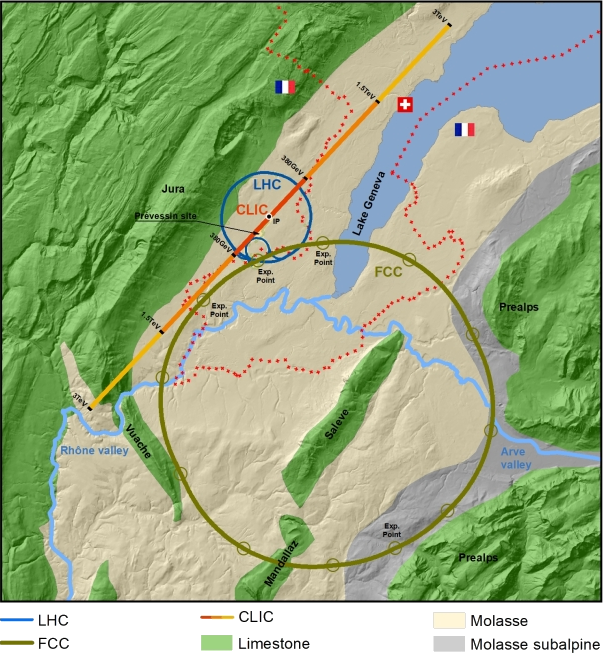
\includegraphics[width=\linewidth]{figures/FCC_CLIC.png}
    \vspace{-10mm}
    \tiny{Image: \href{https://alumni.cern/news/226282}{CERN}}

    \column{.4\textwidth}
    European Particle Physics Strategy:
    \begin{itemize}
      \item Investigate feasibility for FCC at CERN
      \item Hadron collider: $\sqrt{s} = 100$~TeV
      \item Electron-positron collider as first step
      \item Global endeavor
    \end{itemize}
  \end{columns}
\end{frame}

\begin{frame}
  \frametitle{FCC-ee: Lepton Collider}

  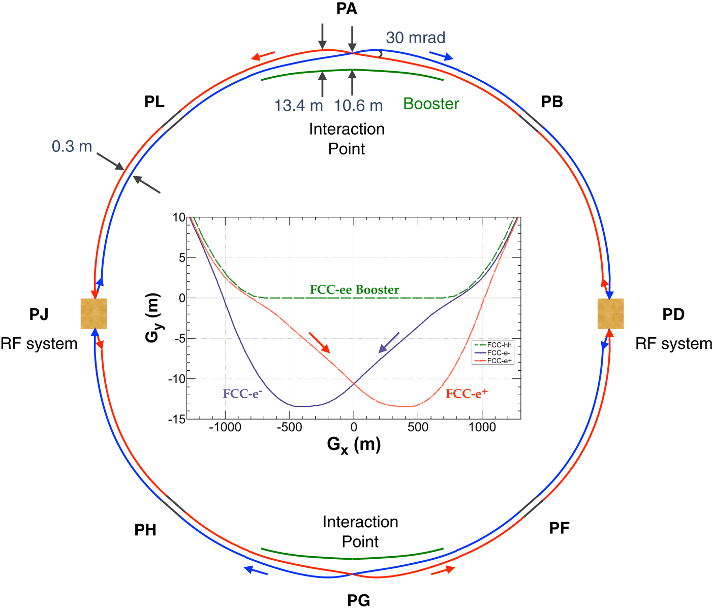
\includegraphics[width=.49\linewidth]{figures/FCC_ee_ring.png}
  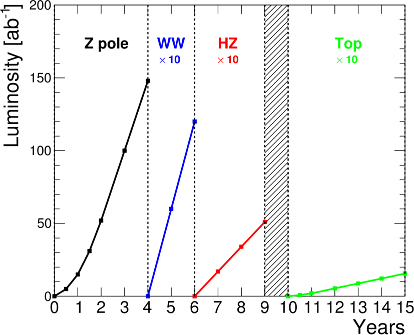
\includegraphics[width=.49\linewidth]{figures/FCC_ee_operation_plan.png}

  FCC-ee characteristics:
  \begin{columns}[c]
    \column{.5\textwidth}
    \begin{itemize}
      \item For precision physics
      \item Higs factory
      \item Electroweak precision $10^{-3} \rightarrow 10^{-5}$
    \end{itemize}

    \column{.5\textwidth}
    \begin{itemize}
      \item Operation at four energies
      \item Clean environment
      \item ``Continuous'' beams
    \end{itemize}
  \end{columns}
\end{frame}

\begin{frame}
  \frametitle{FCC-hh: Hadron Collider}

  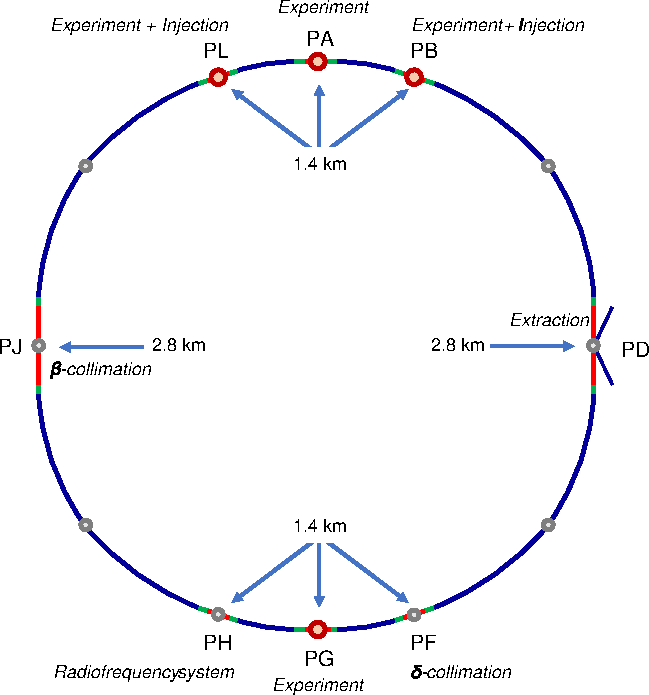
\includegraphics[width=.49\linewidth]{figures/FCC_hh_ring.pdf}
  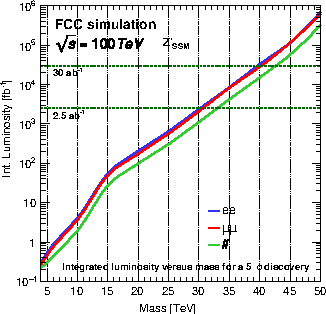
\includegraphics[width=.49\linewidth]{figures/FCC_hh_Zprime_ll.pdf}

  FCC-hh characteristics:

  \begin{columns}[c]
    \column{.5\textwidth}
    \begin{itemize}
      \item Continuation of energy frontier
    \end{itemize}

    \column{.5\textwidth}
    \begin{itemize}
      \item Operation at 100 TeV energies
    \end{itemize}
  \end{columns}
\end{frame}


% ---------------------------------------------------------------------------- %
\section{FCC Detectors}

\begin{frame}
  \frametitle{FCC Detectors}

\end{frame}


% ---------------------------------------------------------------------------- %
\section{Conclusions and Plans}

\begin{frame}
  \frametitle{Conclusions and Plans}

  \begin{itemize}
    \item Upper limit on IC in proton set with 68\% CL at
          $w_\mathrm{u.l.} = 2\%$
    \item Scale uncertainty is the dominant uncertainty
    \item Measurement uncertainty dominated by light jet fraction uncertainty
    \item Combined QCD exhibits lack of compatibility
    \item IC contribution to $\gamma(Z) + c$-jet at 13 TeV is smaller
          \begin{itemize}
            \item Increase only around 30\% for $w = 3.5\%$
            \item Smaller contribution of Compton scattering
          \end{itemize}
  \end{itemize}
\end{frame}

% \appendix
% \backupbegin{}
%
% \begin{frame}
%   \frametitle{Backup}
% \end{frame}
%
% \backupend{}

\end{document}
